In this section, we examine the effective frequency response induced by translation via the time-frequency interpolation method as a function of source azimuth.
As described in \secref{sec:06_Simulation_Framework:Azimuth_Dependence}, for these simulations, we pick $\Delta = 0.5$~m and $s_0 = 2.5$~m (so $\gamma = 10$), and interpolate to $\vec{r}_0 = (0, 0, 0)$.
(Recall that these quantities are defined in \secref{sec:06_Simulation_Framework:Linear_Geometry} for a linear array geometry.)

The induced frequency responses are plotted in \figref{fig:09_Thiergart_Comparison:Azimuth_Dependence} for both the time-frequency interpolation method and our proposed parametric interpolation method (see \chapref{chap:08_Proposed_Method}).
From \figref{fig:09_Thiergart_Comparison:Azimuth_Dependence:Thiergart}, we see that the time-frequency interpolation method tends to produce a comb-filtering response, similar to that of the weighted average method (see \figref{fig:08_Proposed_Method:XF_CombFiltering}), but with much shallower notches.

\begin{figure*}[t]
  \centering
  \begin{subfigure}[b]{0.49\textwidth}
    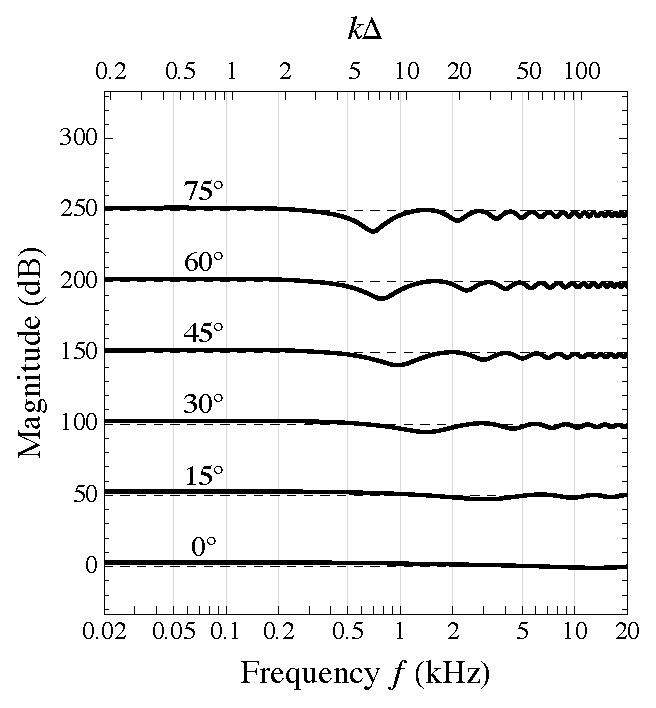
\includegraphics[width=\textwidth]{09_thiergart_comparison/figures/sourceAz_freqResp_thiergart.eps}
    \caption{\citet{Thiergart2013} method}
    \label{fig:09_Thiergart_Comparison:Azimuth_Dependence:Thiergart}
  \end{subfigure}
  \hfill
  \begin{subfigure}[b]{0.49\textwidth}
    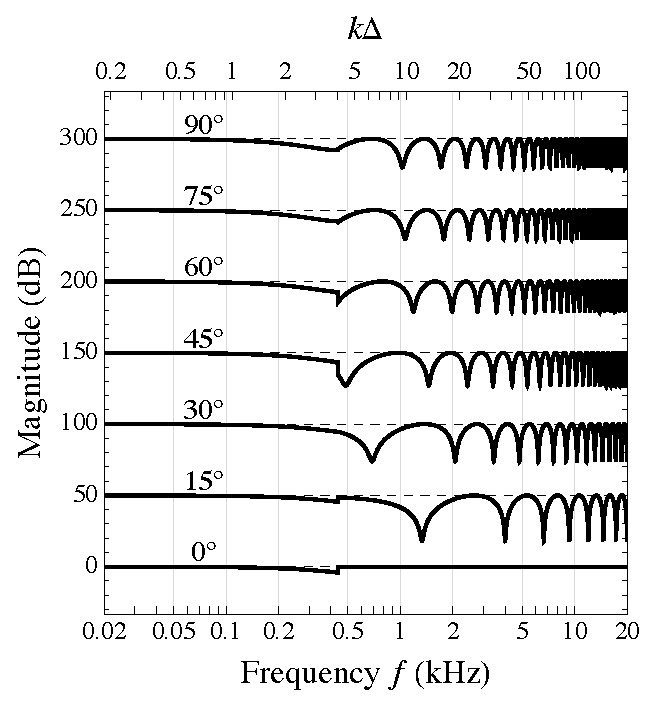
\includegraphics[width=\textwidth]{08_proposed_method/figures/sourceAz_freqResp_validhybrid.eps}
    \caption{Proposed method}
    \label{fig:09_Thiergart_Comparison:Azimuth_Dependence:Hybrid}
  \end{subfigure}

  \caption[Magnitude responses across azimuths for each interpolation method.]{
  Magnitude responses caused by the time-frequency and proposed interpolation methods for various source azimuths.
  The bottom axes show frequency in kHz while the top axes show the nondimensional frequency $k\Delta$ for a microphone spacing of $\Delta = 0.5$~m.
  For legibility, each frequency response is offset by $50$~dB and the responses have been artificially truncated (where needed) to not exceed $-45$~dB.
  \Figref{fig:09_Thiergart_Comparison:Azimuth_Dependence:Hybrid} has been reproduced from \figref{fig:08_Proposed_Method:Azimuth_Dependence:Hybrid}.}
  \label{fig:09_Thiergart_Comparison:Azimuth_Dependence}
\end{figure*} %%NOTE%% vertical axis label is too complicated: |A0 / B0ref| or something

These notches also tend to be wider and spaced farther apart than those of the the comb-filtering response.
Consequently, they may in fact lead to comparably-perceptible coloration, as it is well-established that wider notches are more audible than narrow ones \citep{Bucklein1981}.
Correspondingly, in terms of the computed spectral error (see \eqnref{eq:ABSE}), a wide but shallow notch may yield a comparable spectral error as does a narrow but deep notch once averaged over frequency (due to the effective spectral ``smoothing'' that results from the bank of gammatone filters).

As discussed in \secref{sec:08_Proposed_Method:Azimuth_Dependence}, the frequency response induced by translation via the proposed method (shown in \figref{fig:09_Thiergart_Comparison:Azimuth_Dependence:Hybrid}) consists of a largely flat response at low frequencies concatenated with a comb-filter response at high frequencies.
Psychoacoustic studies have shown that comb-filter responses can be imperceptible if the time-delay between the primary and secondary signals is long enough and/or if their relative levels are different enough \citep{Kates1984,Brunner2007}.
As a result, even though the comb-filter notches shown in \figref{fig:09_Thiergart_Comparison:Azimuth_Dependence:Hybrid} are significantly deeper than those shown in \figref{fig:09_Thiergart_Comparison:Azimuth_Dependence:Thiergart}, it is not necessarily the case that the former will yield more audible coloration than the latter.
This issue will be explored specifically in the following section.
%Ultimately, subjective listening tests may be needed to definitively establish the audibility of the particular colorations induced by each method.

%It should be emphasized that the above plots only illustrate a single condition ($\Delta = 0.5$~m, $\gamma = 10$, and $\vec{r}_0 = (0,0,0)$), so a more comprehensive exploration is required, as will be presented in the following section.